\documentclass[a4paper,10pt]{article}
\usepackage[utf8]{inputenc}
\usepackage[a4paper,top=1in,bottom=1in,right=1in,left=1.5in]{geometry}
\usepackage{amsmath}
\usepackage{anyfontsize}
\usepackage{graphicx}
\usepackage{hyperref}
\usepackage{color}

\begin{document}
\begin{titlepage}
\centering
\vfill
\textbf{\Huge{EEP773
\linebreak
\\Telecommunication\vskip0.18cm
Software Lab}
}\\
\vspace{2cm}
\textbf{\Large{Assignment No. 9}}\\
\textbf{\Large{24 September 2014}}
\vskip2cm
Submitted By:-
\Large{\textbf{\\Paranandi Roopesh
\\2014JTM2264}}
\vskip4cm

\includegraphics[scale=0.05]{iit_logo}\\
\textbf{
Indian Institute of Technology, Delhi
}
\vfill
\end{titlepage}

\tableofcontents
\pagebreak
\listoffigures
\pagebreak
\section{Problem Statement}
\begin{itemize}
 \item The Problem statement was given that using python analyze the contents given in which the conversation between users were given and to analyze the mood of the each user and the percentage of each mood among the users.
\item The mood description should be according to the dictionary given
\item The contents and dictionary should be forked from the given repository and then to work on the forked repository
\end{itemize}
\pagebreak
\section{Assumptions}
These are the following assumptions that are made during the program
\begin{itemize}
 \item The user types his emoticon seperately as a word
 \item In case the user has same number of the emoticons corresponding to more than one mood the mood of the user is decided in the order given in the dictionary
 \item The number of users sending the messages is fixed
\end{itemize}

\pagebreak

\section{Logic}
The program was implemented in the following logical steps
\subsection{forking the given repository}
The repository
\subsection{Reading the contents file word by word}
The contents file is read word by word and if the emoticon is recoginized the corresponding the count which is tracking the emoticon of a particular user is updated
\subsection{Detecting the mood of the user based upon his/her emoticons}
After analyzing the number of emoticons corresponding to each mood the user has used in his conversations, the mood of each user is identified based on which emoticons corresponding to each mood the user has used in his conversations.
\subsection{Analyzing the percentage of each moods}
After analyzing the data about each user percentage of each mood among all the users is calculated
\pagebreak
\pagebreak
\section{output}
The following snapshots shows various outputs.
\begin{figure}[h]
 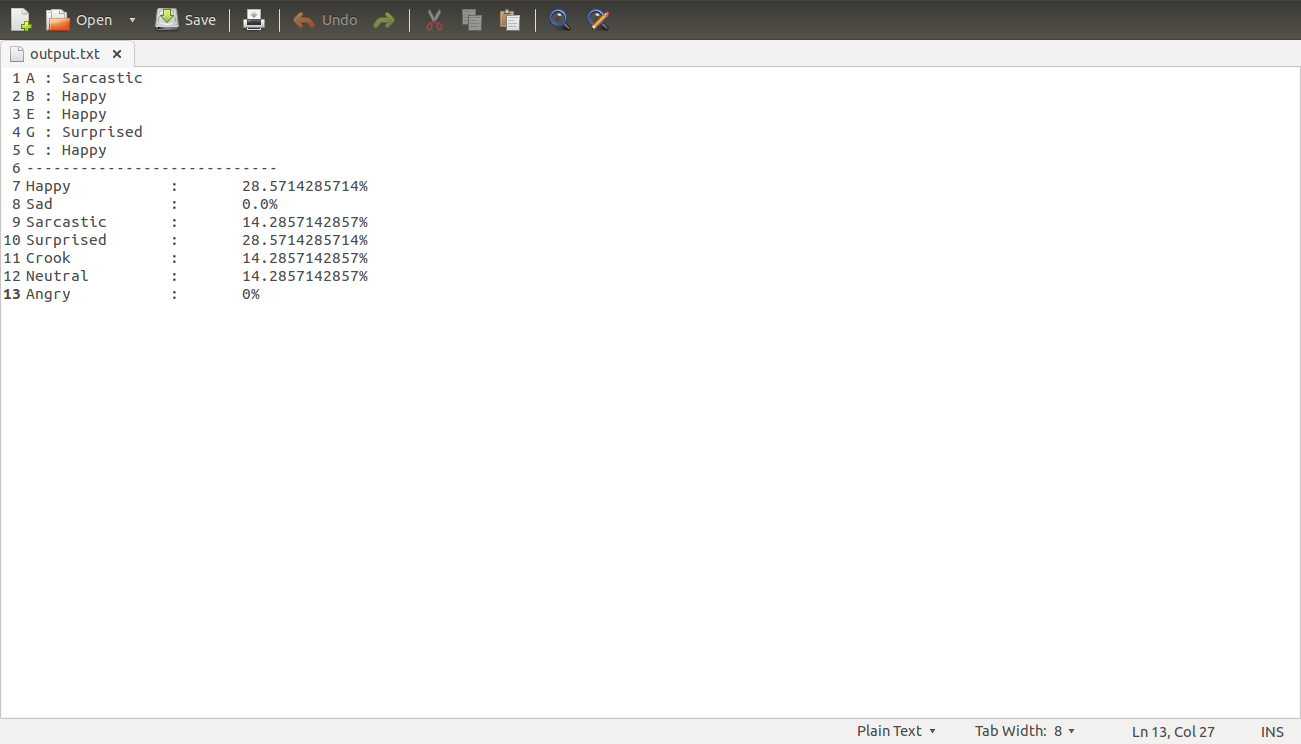
\includegraphics[scale=0.3]{1.png}
 \caption{Image displaying the output}
 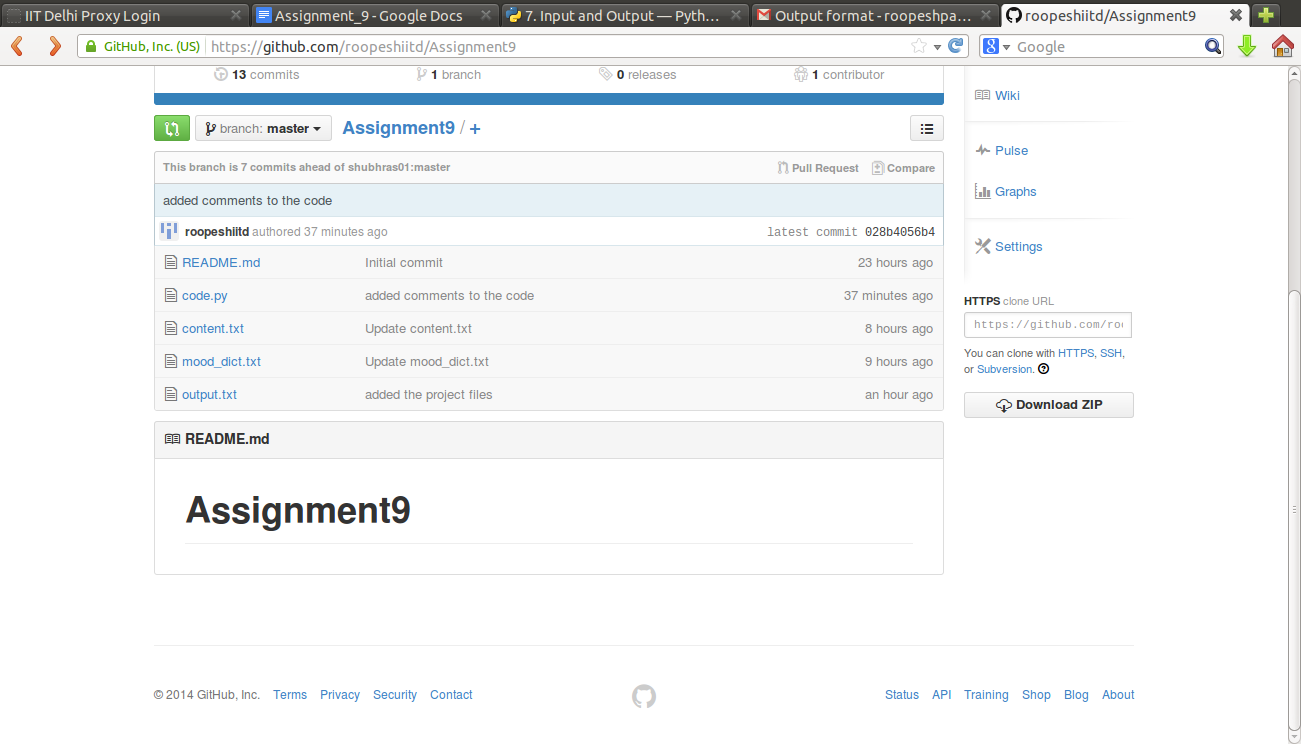
\includegraphics[scale=0.3]{2.png}
 \caption{Image displaying the contents after pushing from local repository to github repository}
\end{figure}



\pagebreak
\pagebreak[3]
\section{References}
\begin{itemize}
 \item www.tutorialspoint.com
 \item Python for dummies 
 \item http://developers.google.com/tutotial/python
 \item www.stackoverflow.com
\end{itemize}

\end{document}
